\begin{center}
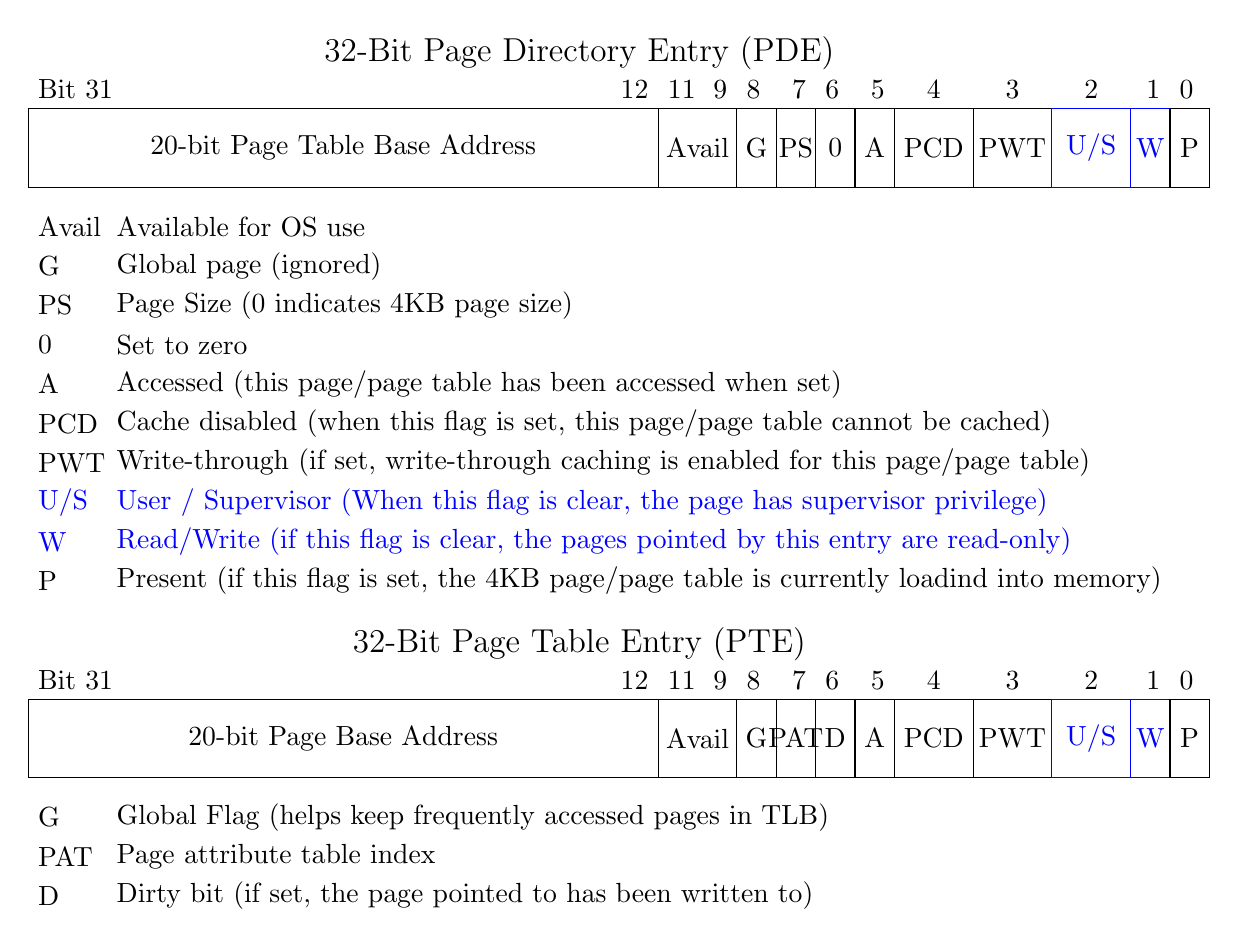
\begin{tikzpicture}
\draw node at (7,1.7) {{\large 32-Bit Page Directory Entry (PDE)}};
\draw (0,0) rectangle (8,1) node [pos = 0.5] {20-bit Page Table Base Address};
\draw (8,0) rectangle (9,1) node [pos = 0.5] {Avail};
\draw (9,0) rectangle (9.5,1) node [pos = 0.5] {G};
\draw (9.5,0) rectangle (10,1) node [pos = 0.5] {PS};
\draw (10,0) rectangle (10.5,1) node [pos = 0.5] {0};
\draw (10.5,0) rectangle (11,1) node [pos = 0.5] {A};
\draw (11,0) rectangle (12,1) node [pos = 0.5] {PCD};
\draw (12,0) rectangle (13,1) node [pos = 0.5] {PWT};
\draw [blue] (13,0) rectangle (14,1) node [pos = 0.5] {U/S};
\draw [blue] (14,0) rectangle (14.5,1) node [pos = 0.5] {W};
\draw (14.5,0) rectangle (15,1) node [pos = 0.5] {P};

\draw node at (0,1) [above right] {Bit 31};
\draw node at (8,1) [above left] {12};
\draw node at (8,1) [above right] {11};
\draw node at (9,1) [above left] {9};
\draw node at (9,1) [above right] {8};
\draw node at (10,1) [above left] {7};
\draw node at (10,1) [above right] {6};
\draw node at (11,1) [above left] {5};
\draw node at (11.5,1) [above] {4};
\draw node at (12.5,1) [above] {3};
\draw node at (13.5,1) [above] {2};
\draw node at (14.5,1) [above left] {1};
\draw node at (14.5,1) [above right] {0};

\draw node at (0,-0.5) [right] {Avail};
\draw node at (1,-0.5) [right] {Available for OS use};
\draw node at (0,-1) [right] {G};
\draw node at (1,-1) [right] {Global page (ignored)};
\draw node at (0,-1.5) [right] {PS};
\draw node at (1,-1.5) [right] {Page Size (0 indicates 4KB page size)};
\draw node at (0,-2) [right] {0};
\draw node at (1,-2) [right] {Set to zero};
\draw node at (0,-2.5) [right] {A};
\draw node at (1,-2.5) [right] {Accessed (this page/page table has been accessed when set)};
\draw node at (0,-3) [right] {PCD};
\draw node at (1,-3) [right] {Cache disabled (when this flag is set, this page/page table cannot be cached)};
\draw node at (0,-3.5) [right] {PWT};
\draw node at (1,-3.5) [right] {Write-through (if set, write-through caching is enabled for this page/page table)};
\draw [blue] node at (0,-4) [right] {U/S};
\draw [blue] node at (1,-4) [right] {User / Supervisor (When this flag is clear, the page has supervisor privilege)};
\draw [blue] node at (0,-4.5) [right] {W};
\draw [blue] node at (1,-4.5) [right] {Read/Write (if this flag is clear, the pages pointed by this entry are read-only)};
\draw node at (0,-5) [right] {P};
\draw node at (1,-5) [right] {Present (if this flag is set, the 4KB page/page table is currently loadind into memory)};

\draw node at (7,-5.8) {{\large 32-Bit Page Table Entry (PTE)}};
\draw (0,-7.5) rectangle (8,-6.5) node [pos = 0.5] {20-bit Page Base Address};
\draw (8,-7.5) rectangle (9,-6.5) node [pos = 0.5] {Avail};
\draw (9,-7.5) rectangle (9.5,-6.5) node [pos = 0.5] {G};
\draw (9.5,-7.5) rectangle (10,-6.5) node [pos = 0.5] {PAT};
\draw (10,-7.5) rectangle (10.5,-6.5) node [pos = 0.5] {D};
\draw (10.5,-7.5) rectangle (11,-6.5) node [pos = 0.5] {A};
\draw (11,-7.5) rectangle (12,-6.5) node [pos = 0.5] {PCD};
\draw (12,-7.5) rectangle (13,-6.5) node [pos = 0.5] {PWT};
\draw [blue] (13,-7.5) rectangle (14,-6.5) node [pos = 0.5] {U/S};
\draw [blue] (14,-7.5) rectangle (14.5,-6.5) node [pos = 0.5] {W};
\draw (14.5,-7.5) rectangle (15,-6.5) node [pos = 0.5] {P};

\draw node at (0,-6.5) [above right] {Bit 31};
\draw node at (8,-6.5) [above left] {12};
\draw node at (8,-6.5) [above right] {11};
\draw node at (9,-6.5) [above left] {9};
\draw node at (9,-6.5) [above right] {8};
\draw node at (10,-6.5) [above left] {7};
\draw node at (10,-6.5) [above right] {6};
\draw node at (11,-6.5) [above left] {5};
\draw node at (11.5,-6.5) [above] {4};
\draw node at (12.5,-6.5) [above] {3};
\draw node at (13.5,-6.5) [above] {2};
\draw node at (14.5,-6.5) [above left] {1};
\draw node at (14.5,-6.5) [above right] {0};

\draw node at (0,-8) [right] {G};
\draw node at (1,-8) [right] {Global Flag (helps keep frequently accessed pages in TLB)};
\draw node at (0,-8.5) [right] {PAT};
\draw node at (1,-8.5) [right] {Page attribute table index};
\draw node at (0,-9) [right] {D};
\draw node at (1,-9) [right] {Dirty bit (if set, the page pointed to has been written to)};
\end{tikzpicture}
\end{center}